\documentclass[12pt, a4paper, twoside]{article}
\usepackage[utf8]{inputenc}
\usepackage[cm]{fullpage}
\usepackage{fancyhdr}
\usepackage{textcomp}
\usepackage{graphicx}
\usepackage{commath}
\usepackage[portuguese]{babel}
\usepackage{float}
\usepackage{hyperref}

\begin{document}

\title{Pré-relatório 4 do Laboratório de Dispositivos e Circuitos Eletrônicos}
\author{Cristiano Silva Júnior: 13/0070629}
\date{\today}
\maketitle

Neste relatório, vamos utilizar três modelos para o diodo. O primeiro deles é o modelo ideal, em que o diodo é um circuito fechado para quedas de tensão positivas e um circuito aberto para quedas de tensão negativas.

\begin{figure}[H]
    \centering
    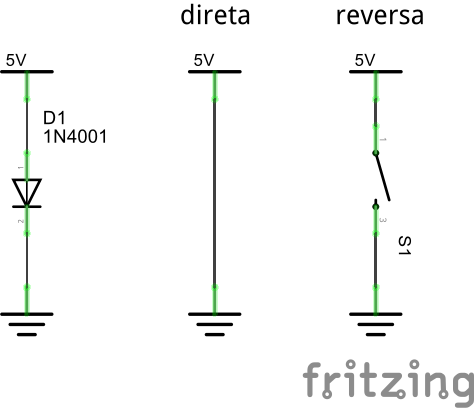
\includegraphics[width=0.4\textwidth]{figs/diode.png}
    \caption{Modelo ideal do diodo}
\end{figure}

O segundo modelo a ser utilizado é o modelo de queda de tensão constante, em que o diodo passa a ser um diodo ideal com uma fonte de tensão em série. Neste caso, o diodo somente conduz para tensões maiores do que a sua tensão de polarização.

\begin{figure}[H]
    \centering
    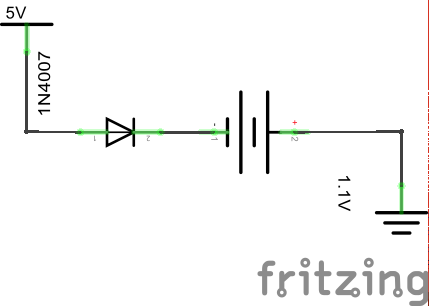
\includegraphics[width=0.4\textwidth]{figs/diode2.png}
    \caption{Modelo de tensão constante do diodo}
\end{figure}

Neste modelo, podemos levar em conta o efeito Zener, em que, para alguns diodos, o diodo também conduz para quedas de tensão muito negativas. No caso, um diodo com características de Zener conduz também para tensões menores que a sua tensão de Zener.

O terceiro modelo é o chamado diodo real, em que a corrente $i$ que passa pelo diodo depende da tensão $V$ aplicada sobre ele:
$$i = I_s\left( e^{\frac{V}{nV_T}} - 1 \right)$$

\section{Exercício 1}

\begin{figure}[H]
    \centering
    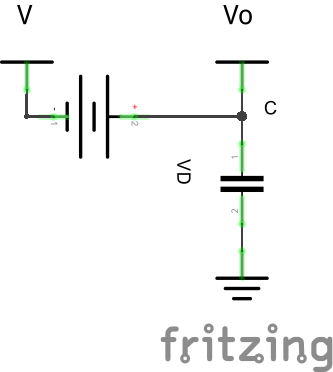
\includegraphics[width=0.4\textwidth]{figs/rel4/ex1.png}
    \caption{Diagrama com modelo de tensão constante no diodo para condução direta.}
\end{figure}

Utilizando o modelo de tensão constante do diodo para resolver o circuito proposto, podemos atualizar o diagrama, como desenhado na figura 3. Neste caso, é possível que a saída, em regime permanente, será uma tensão DC $v_o = V_p - V_D$, onde $V_D$ é a queda de tensão do diodo.

\section{Exercício 2}

\begin{figure}[H]
    \centering
    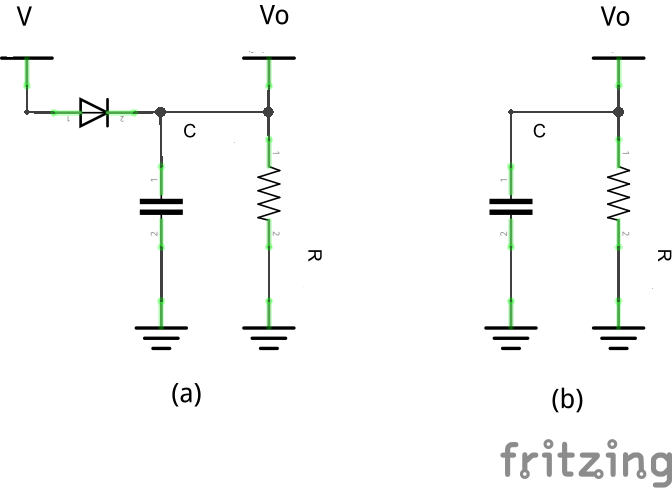
\includegraphics[width=0.8\textwidth]{figs/rel4/ex2.png}
    \caption{(a) Circuito com diodo em modo de condução. (b) Circuito com diodo em polarização reversa. Neste caso, o diodo é tratado como um circuito aberto, restando somente o circuito RC.}
\end{figure}

Analisando a corrente $i_L$ da carga no circuito em questão, nota-se que a saída terá uma forma de onda similar a saída, mas com valor máximo $i_{Lmax} = \frac{V_P}{R_L}$. Isto é, ela acompanhará a senoide da entrada quando crescer mas, quando a entrada começar a decair, devido ao capacitor, a tensão no resistor decairá vagarosamente, não chegando a se anular até encontrar uma tensão de crescimento da entrada novamente. Desta forma, a saída é similar a uma tensão DC, com algumas variações.

\section{Exercício 3}

Neste laboratório, utilizaremos o diodo $1N4739$, que é caracterizado por ser um diodo Zener para aplicações de potência. Analisando o \textit{datasheet} do componente fornecido pela \textit{Fairchild Semiconductors}, podemos estudar alguns de seus valores nominais:

\begin{itemize}
    \item Tensão de Zener $V_Z = 9,1V$ a corrente de Zener $I_Z = 28ma$;
    \item Máxima impedância $Z_Z = 5 \Omega$;
\end{itemize}

\section{Exercício 4}

Resolvendo o problema utilizando o procedimento de Sedra et al. (2014), primeiro determinamos qual o estado do diodo em uma região de mínima condução. Depois descobrimos a queda de tensão no diodo com o modelo naquele estado dentro do circuito. Por fim, descobrimos um resistor de carga que garanta aquela mesma queda de queda de tensão no ponto selecionado no circuito. Desta forma, garantimos que a corrente no diodo é menor do que a necessária para conduzir com aquela tensão.

Assumimos que a tensão $V_Z$ sobre o diodo é dada pela tensão sobre a impedância de Zener somada à tensão de Zener $V_{Zo}$. Sendo assim,
$$ V_Z = V_{Zo} + Z_Z \cdot I_Z \Leftrightarrow V_{Zo} = V_z - Z_Z \cdot I_Z $$

\begin{figure}[H]
    \centering
    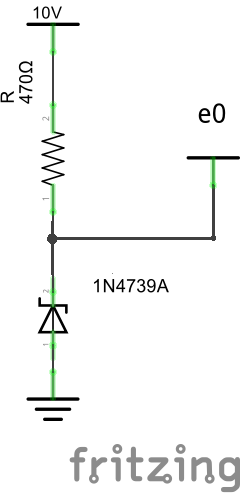
\includegraphics[width=0.4\textwidth]{figs/rel4/ex4-1.png}
    \caption{Circuito somente com diodo montado}
\end{figure}

Montando o diodo no circuito, temos que a corrente agora será
$$ I_Z = \frac{V-V_{Zo}}{R+Z_Z} $$
$$ \Rightarrow e_0 = V - I_Z \cdot R $$

Agora sem o diodo no circuito, vamos encontrar um valor $R_L$ para o resistor de carga que garanta esta queda de tensão:

\begin{figure}[H]
    \centering
    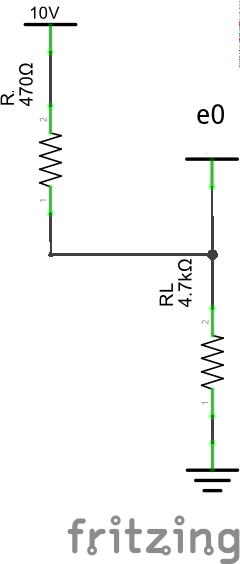
\includegraphics[width=0.4\textwidth]{figs/rel4/ex4-2.png}
    \caption{Circuito somente com resistor de carga}
\end{figure}

Por divisor de tensão,
$$ e_0 = V \cdot \frac{R_L}{R_L+R} $$
$$ \Leftrightarrow R_L = \frac{e_0 \cdot R}{V-e_0s} $$
Numericamente,
$$ R_L = 4355,769 \Omega $$

\section{Exercício 5}

Para uma aplicação real, o circuito proposto no exercício, que pode ser visto na figura 6 deste relatório, não pode ser utilizado como uma fonte de tensão DC, já que há uma variação muito grande em sua saída para ser considerado uma fonte DC.

Além disso, por questões de segurança, espera-se que a impedância nas saídas de um componente como este seja nula, e logo se nota que a impedância é, considerando o transformador como ideal, $Z = \frac{1}{\jmath C \omega}$, onde $\omega = 120 \pi$ radianos, para o sistema energético brasileiro.

\section{Exercício 6}

Assumindo o transformador utilizado no problema como ideal, espera=se que a sua frequência de saída seja igual à frequência da linha. Neste caso, como a energia elétrica no Brasil é transmitida a $60Hz$, então a frequência de excitação do circuito é de $60Hz$.

\section{Exercício 7}

O valor RMS de uma medida $V$ é definida como
$$ V_{RMS} = \left( \frac{1}{T} \int_0^T V(t)^2 \mathrm{d}t \right)^{\frac{1}{2}} $$
onde $T$ é o período da onda que descreve $V$. No nosso caso,
$$ V(t) = A \sin(2 \pi f t) $$
pois esperamos este formato na energia fornecida pelo sistema energético brasileiro. Substituindo $V$ na definição do valor RMS, notamos que
$$ V_{RMS} = \frac{A}{\sqrt{2}} $$
Como no problema $V_{RMS} = 12V$, então o valor de pico da tensão será
$$ A = \sqrt{2} \cdot V_{RMS} = 16.97V $$

\section{Exercício 8}

A tensão de ondulação (ou de \textit{ripple}) é a variação (geralmente residual e indesejada) de uma fonte de tensão DC. Ela surge quando há uma fonte de tensão DC feita a partir de uma fonte de tensão AC.

\section{Exercício 9}

Segundo Chen et al. (2017), para um retificador de onda completa construído como o descrito no experimento em questão, a queda de tensão pico a pico de \textit{ripple} sobre o capacitor é $$V_{pp} = \frac{I}{2fC}$$ onde $I$ é a corrente que passa pelo dispositivo; e $f$ é a frequência de linha utilizada para montar o retificador.

\section{Exercício 10}

Pela lei de Ohm, a tensão sobre um componente resistor é $V=RI$. Logo, se espera que, quanto menor a resistência, menor a tensão sobre ele.

\section{Exercício 11}

Este diodo Zener foi colocado na função de regular tensão. Este é um dos vários usos deste componente, e, quando ele é utilizado desta forma, o circuito geralmente contém um resistor em paralelo com o diodo (Sedra et al., 2014).

\section{Exercício 12}

Um circuito regulador tem como premissa a regulação da tensão sobre ele para que ela se mantenha constante. Em geral, ele construído com um circuito retificador seguido de alguns filtros à escolha do fabricante, já que o retificador não tem uma saída constante, como comentado no exercício 5 deste pré-relatório.

\section{Referência Bibliográfica}

\begin{itemize}
    \item SEDRA, Adel. SMITH, Kenneth. "Microelectronic Circuits."  Oxford University Press, 7th edition, 2014.
    \item CHEN, Lei. GÖTTING, Gunther. HAHN, Ingo. "DC-Link Current and Torque Ripple Optimized Self-Sensing Control of Interior Permanent-Magnet Synchronous Machines for Hybrid and Electrical Vehicles." IEEE Transactions on Industry Applications. Volume 53, Issue 5, 2017.
    \item Fairchild Instruments. "1N4739A: Zener 9.1V 1W 5\%". Disponível em \url{http://www.onsemi.com/PowerSolutions/product.do?id=1N4739A}. Acesso em 25 de Setembro de 2017.
    \item Notas de aula do professor Geovanny.
\end{itemize}

\end{document}
